\documentclass{article}
\usepackage{amsmath} %Never write a paper without using amsmath for its many new commands
\usepackage{amssymb} %Some extra symbols
\usepackage{makeidx} %If you want to generate an index, automatically
\usepackage{graphicx} %If you want to include postscript graphics
%%%  \usepackage{mystyle} 
%Create your own file, mystyle.sty where you put all your own \newcommand statements
%%%
%%%
\usepackage{amscd}

\usepackage{Sweave}


%%\VignetteIndexEntry{Examples from WINRPACK}

%%% \usepackage{Sweave}

\begin{document}

%%%\renewcommand\floatpagefraction{.9}
%%%\renewcommand\topfraction{.9}
%%%\renewcommand\bottomfraction{.9}
%%%\renewcommand\textfraction{.1}
%%%\setcounter{totalnumber}{50}
%%%\setcounter{topnumber}{50}
%%%\setcounter{bottomnumber}{50}

\setkeys{Gin}{width=0.9\textwidth}



\numberwithin{equation}{section}

%%%   \SweaveOpts{prefix.string=winrpack}



\author{Jonathan M. Lees\\
University of North Carolina, Chapel Hill\\
Department of Geological Sciences\\
CB \#3315, Mitchell Hall\\
Chapel Hill, NC  27599-3315\\
email: jonathan.lees@unc.edu\\
ph: (919) 962-0695
}

\title{WINRPACK: Convert WIN to  R}
\date{MARCH, 2008}

\maketitle


\begin{abstract}
Convert WIN format data from Japan to R
\end{abstract}


\section{Getting started}


Win format data consists of 3 files:
a pick file that has infomation about the arrival times
and the phase arrival picks, 
and two files that store the waveform data.
These are 
a channel file and a digital waveform file.
The channel file is a meta-data file that
has information on how the
waveforms are stored, so they can be extracted by the C-code 
programs.

First read in the pickfile:

\begin{Schunk}
\begin{Sinput}
> library(WINRPACK)
> winpick = "060413.021851.231"
> zip = get1WINPICK(winpick)
\end{Sinput}
\end{Schunk}

This is a list structure that consists of a copy of the pickfile
in WIN format and a break down of the pickfile
after it has been parsed.

The structure is as follows:

\begin{Schunk}
\begin{Sinput}
> names(zip)
\end{Sinput}
\begin{Soutput}
 [1] "PF"     "AC"     "LOC"    "MC"     "REFT"   "STA"    "LIP"    "E"     
 [9] "infile" "winID1" "LEVEL"  "PICKER"
\end{Soutput}
\end{Schunk}

The documentation call will show how this data is
stored in R, for example, help(get1WINPICK),
which will show the list structure 
of the data collected by the conversion program.

\begin{verbatim}
      PF: original pick file
      AC: event card (a-card)
     LOC: location
      yr: year
      jd: julian day
      mo: month
     dom: day or month
      hr: hour
      mi: minute
     sec: sec
     lat: lat
     lon: lon
       z: depth (km)
     mag: magnitude
      MC: focal mechanism card
    REFT: Reference time for phase arrivals
      yr: year
      jd: julian day
      mo: month
     dom: day or month
      hr: hour
      mi: minute
     sec: sec
     STA: List of stations
     tag: id tag for station
    name: station name
    comp: component
      c3: other id tag
    ppol: polarity
    parr: p-aarival time relative to reference
    pflg: flag
    perr: p-error
    pres: p-residual
    sarr: s-arrival time relative to reference
    sflg: flag
    serr: s-error
    sres: s-residual
     LIP: error ellipse
       E: simple error card
  infile: input file name
  winID1: WIN ID number
   LEVEL: level
  PICKER: name of picker
\end{verbatim}

In WIN format the pcikfile contains information on where to 
extract the waveforms.  To read in the waveforms one must first 
get information on the channels stored in the 
binary file.  
On my computer the waveforms and the pickfiles are stored in 
different directories.  This information must be indicated
to the calling program, of course.
The channel file contains information about the stations
and their arrangement in the waveform file.
For this example we have stored the pickfile 
in the local directory
but typically these will be stored on disk
in the a remote directory.
The full path name to the 
pickfile and the waveform file directories
must be supplied to the 
conversion programs. 

Once we read in the pickfile, we extract the 
waveform ID  from the pickfile and
use that to find the correct associated
waveform file.

As an example, we next read in the channel file
to set the LAT-LON coordinates of the stations
recorded on the waveform file.  The program readwinch
is later called again from the program XWINdata,
so this step can often be skipped.


\begin{Schunk}
\begin{Sinput}
> fn = zip$winID1
> chans = readwinch(fn)
> m1 = match(zip$STA$name, chans$sta)
> zip$STA$lat = chans$lat[m1]
> zip$STA$lon = chans$lon[m1]
> zip$STA$z = chans$z[m1]
\end{Sinput}
\end{Schunk}

The next program actually reads in the channel file and then extracts the infromation 
from waveform data file.

\begin{Schunk}
\begin{Sinput}
> JH = XWINdata(fn, stasel = NULL, PLOT = FALSE)
> L = length(JH)
\end{Sinput}
\end{Schunk}

The argument stasel  allows one to select only a subset of traces from the 
WIN data file.

The data is now in memory and it can be used for plotting and other analysis.
For example, suppose I want to view one of the 
traces in the structure.

The structure JH has 80 elements or 80 traces.
Lets consider the first one.  To see the meta data structure,
we print the names of the list:

\begin{Schunk}
\begin{Sinput}
> names(JH[[1]])
\end{Sinput}
\begin{Soutput}
[1] "fn"     "sta"    "comp"   "dt"     "DATTIM" "N"      "units"  "amp"   
\end{Soutput}
\end{Schunk}

We see that the  structure has the meta data and the trace data (the waveform)
in it.
To plot the first trace, we can very simply try:

\begin{Schunk}
\begin{Sinput}
> y = JH[[1]]$amp
> x = seq(from = 0, by = JH[[1]]$dt, length = length(y))
\end{Sinput}
\end{Schunk}

\begin{Schunk}
\begin{Sinput}
> plot(x, y, type = "l", xlab = "sec", ylab = "amplitude", main = paste(JH[[1]]$sta, 
+     JH[[1]]$comp, sep = " "))
\end{Sinput}
\end{Schunk}

The user can make a function to plot part or all of the traces or
do other analysis.

More commonly the pickfiles may be stored
in some remote directory, for example:

\begin{verbatim}
pickdir = '/data/gauss/sake/Fuji/Picks/2001'
wigdir = '/data/gauss/sake/Fuji/Wigs/2001'
\end{verbatim}
The waveforms are further broken down into 
directories by month:
\begin{verbatim}
% ls /data/gauss/sake/Fuji/Wigs/2001
01  02  03  04  05  06  07  08  09  10  11  12
\end{verbatim}
So to extract the correct file name associated with a pickfile,
we must make sure we are pointing to the correct directory.
The zip list has this information in it:
\begin{Schunk}
\begin{Sinput}
> wigdir = paste(sep = "/", "/data/gauss/sake/Fuji/Wigs", zip$LOC$yr, 
+     formatC(zip$LOC$mo, width = 2, flag = "0"))
> testfn = paste(sep = "/", wigdir, zip$winID1)
\end{Sinput}
\end{Schunk}
which can be used to replace the file name ``fn'' in the examples above.

To use the RSEIS software, first convert this structure with a
program to reformat the list into a seismic structure:

\begin{Schunk}
\begin{Sinput}
> require(RSEIS)
> KH = prepSEIS(JH)
\end{Sinput}
\end{Schunk}

All this does is reorganize the data into
a structure used by this package.
Now the data can be plotted and 
analyzed with all the power in the RSEIS package.

\begin{Schunk}
\begin{Sinput}
> w1 = which(KH$COMPS == "V")
> PICK.GEN(KH, sel = w1, SHOWONLY = TRUE)
\end{Sinput}
\end{Schunk}
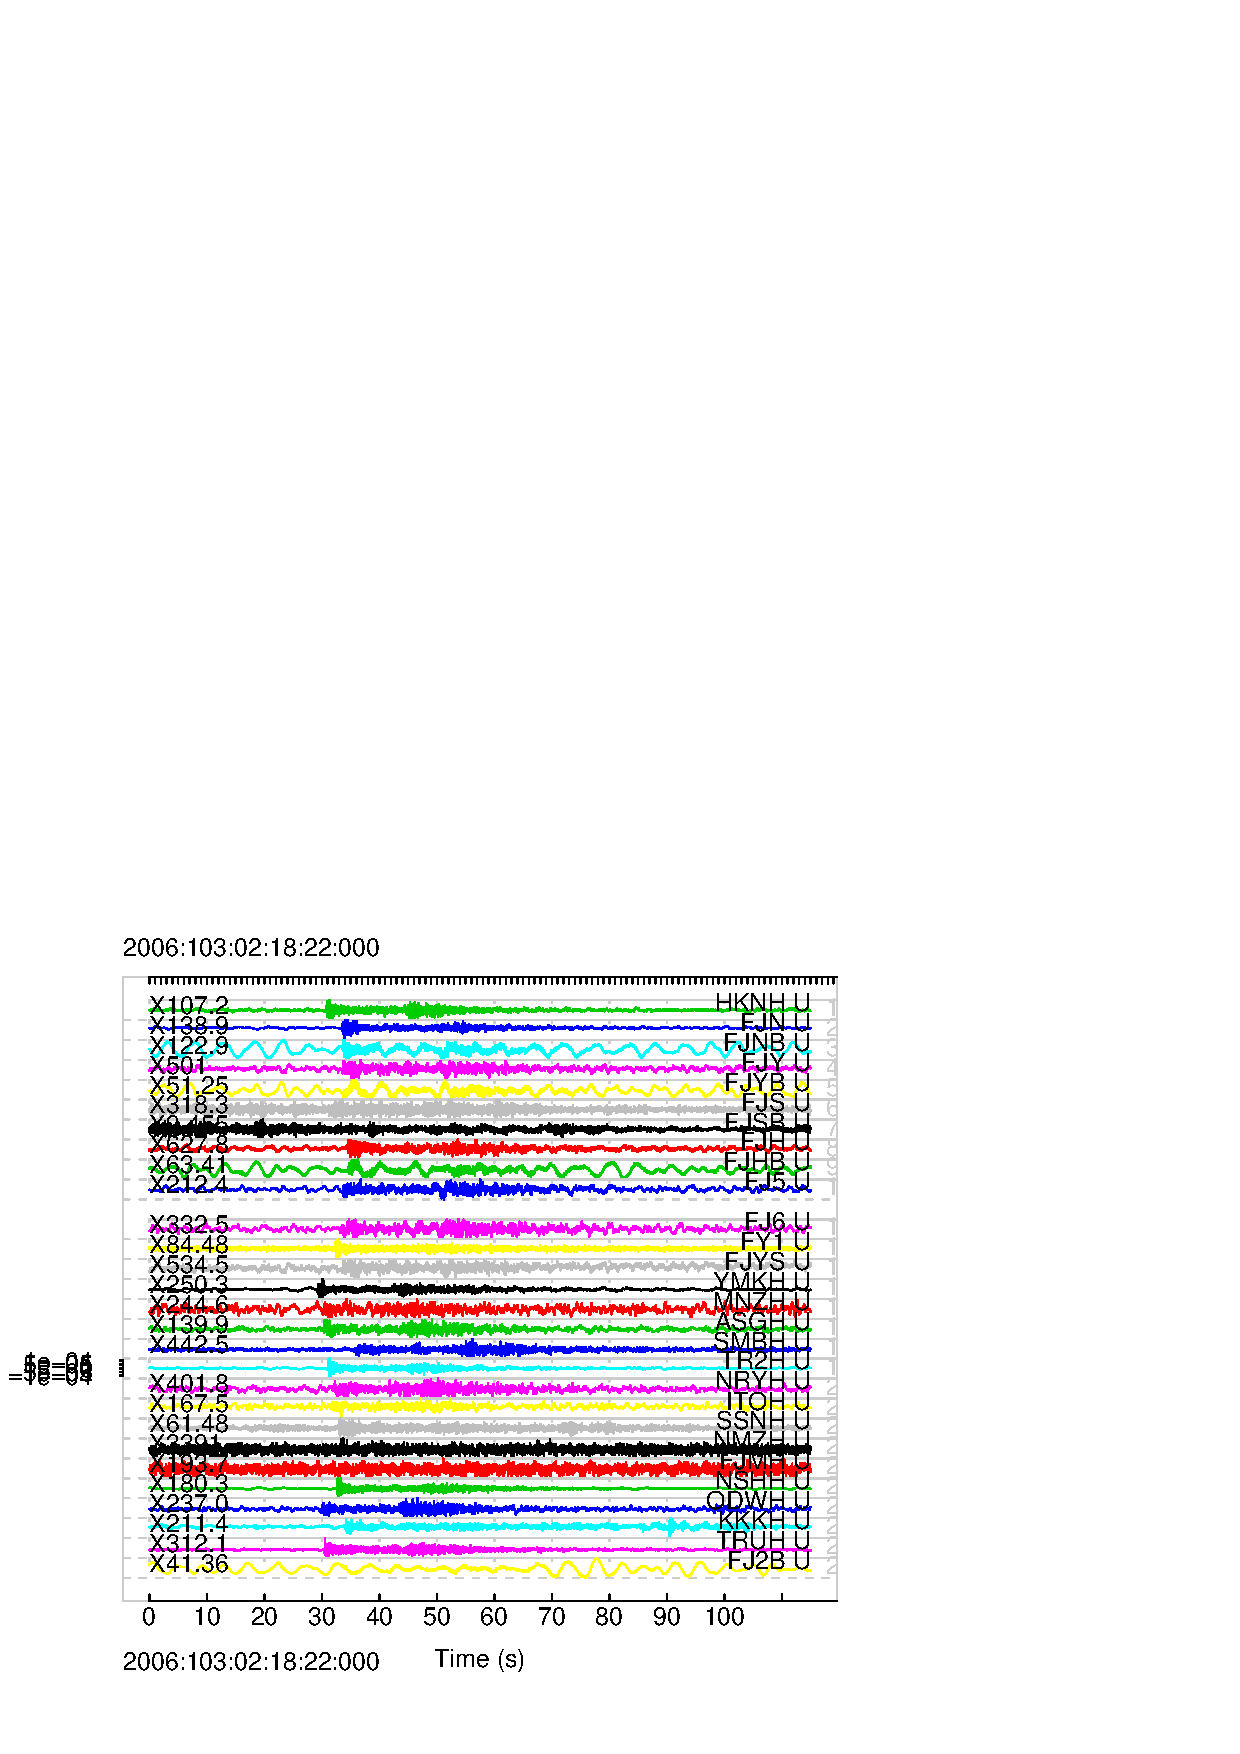
\includegraphics{WIN2R-010}

Not all the traces have associated phase picks.
We can select off the ones that do and plot them
according to arrival time.
To sort these according to the times of the first arrivals one may do something like this:

\begin{Schunk}
\begin{Sinput}
> match(zip$STA$name, KH$STNS[w1])
> w2 = w1[match(zip$STA$name, KH$STNS[w1])]
> B = order(zip$STA$parr)
> PICK.GEN(KH, sel = w2[B], SHOWONLY = TRUE)
\end{Sinput}
\end{Schunk}
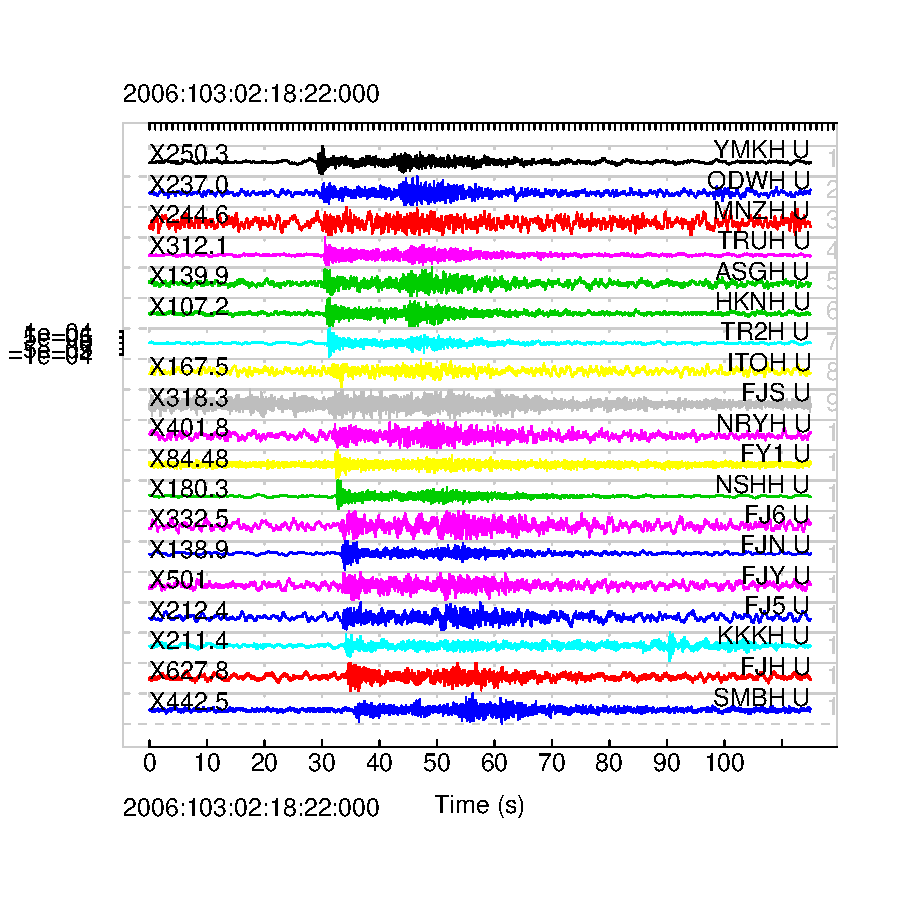
\includegraphics{WIN2R-011}

Finally, to analyze the data using the full power of RSEIS, remove the 
SHOWONLY argument (or set to false) so that the program enters
interactive mode.  Buttons can be accessed this way, but I recommend
looking over the documentation of RSEIS before proceeding.

To see a plot of the station configuration that recorded
the event:
\begin{Schunk}
\begin{Sinput}
> plot(zip$STA$lon, zip$STA$lat, pch = 6, xlab = "LON", ylab = "LAT", 
+     main = zip$winID1)
> segments(zip$STA$lon, zip$STA$lat, zip$LOC$lon, zip$LOC$lat, 
+     col = "red")
> text(zip$STA$lon, zip$STA$lat, labels = zip$STA$name, pos = 3)
\end{Sinput}
\end{Schunk}
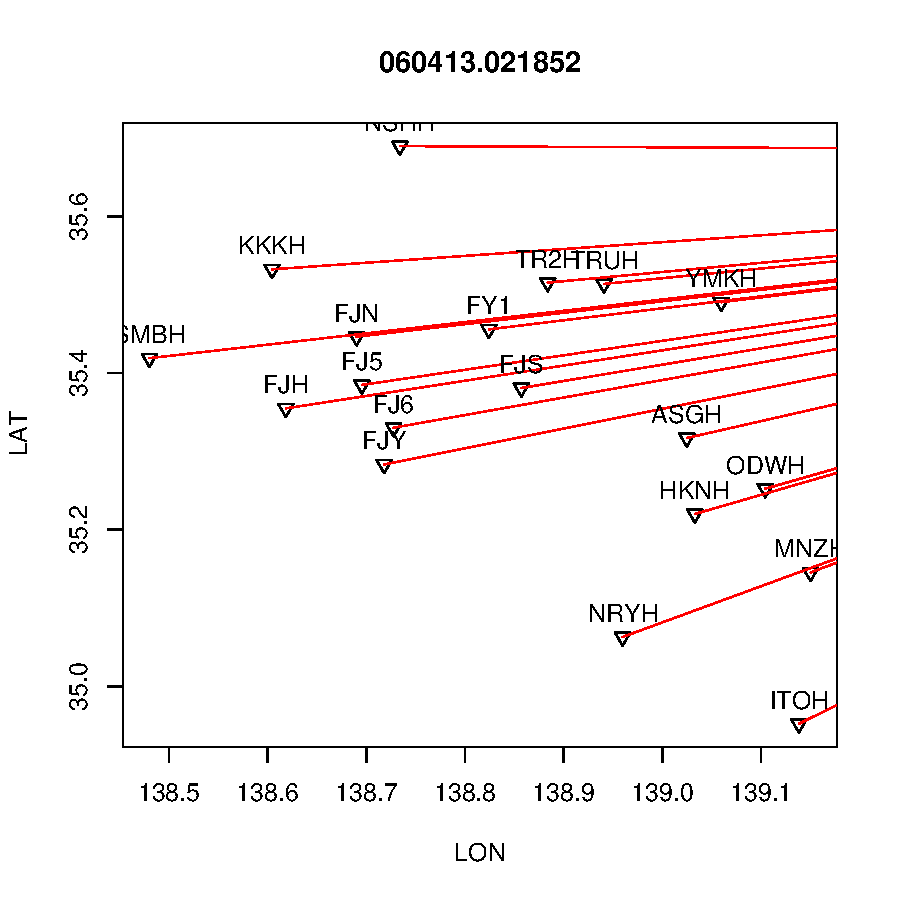
\includegraphics{WIN2R-012}



\end{document}
